\section{Conclusion}
By applying all these methods and combining them in a most profitable way, the Ferienakademie produces impressive results year after year. These are usually presented on the final evening where the courses come together to share their works with their peers. But the courses notwithstanding, this summer school is a complete success. Students with a motivation for holistic learning from a lot of different fields come together for twelve days to work, study and -- most importantly-- have fun together. Ferienakademie succeeds at connecting those aspects which sometimes get lost in regular studies and is a great opportunity for students to reap their benefits. If you are not yet convinced, hopefully these final expressions \autoref{fig:durnholz} and \autoref{fig:Snow} can tip the scale.
\begin{figure}[ht]%
 	\begin{center}%
 		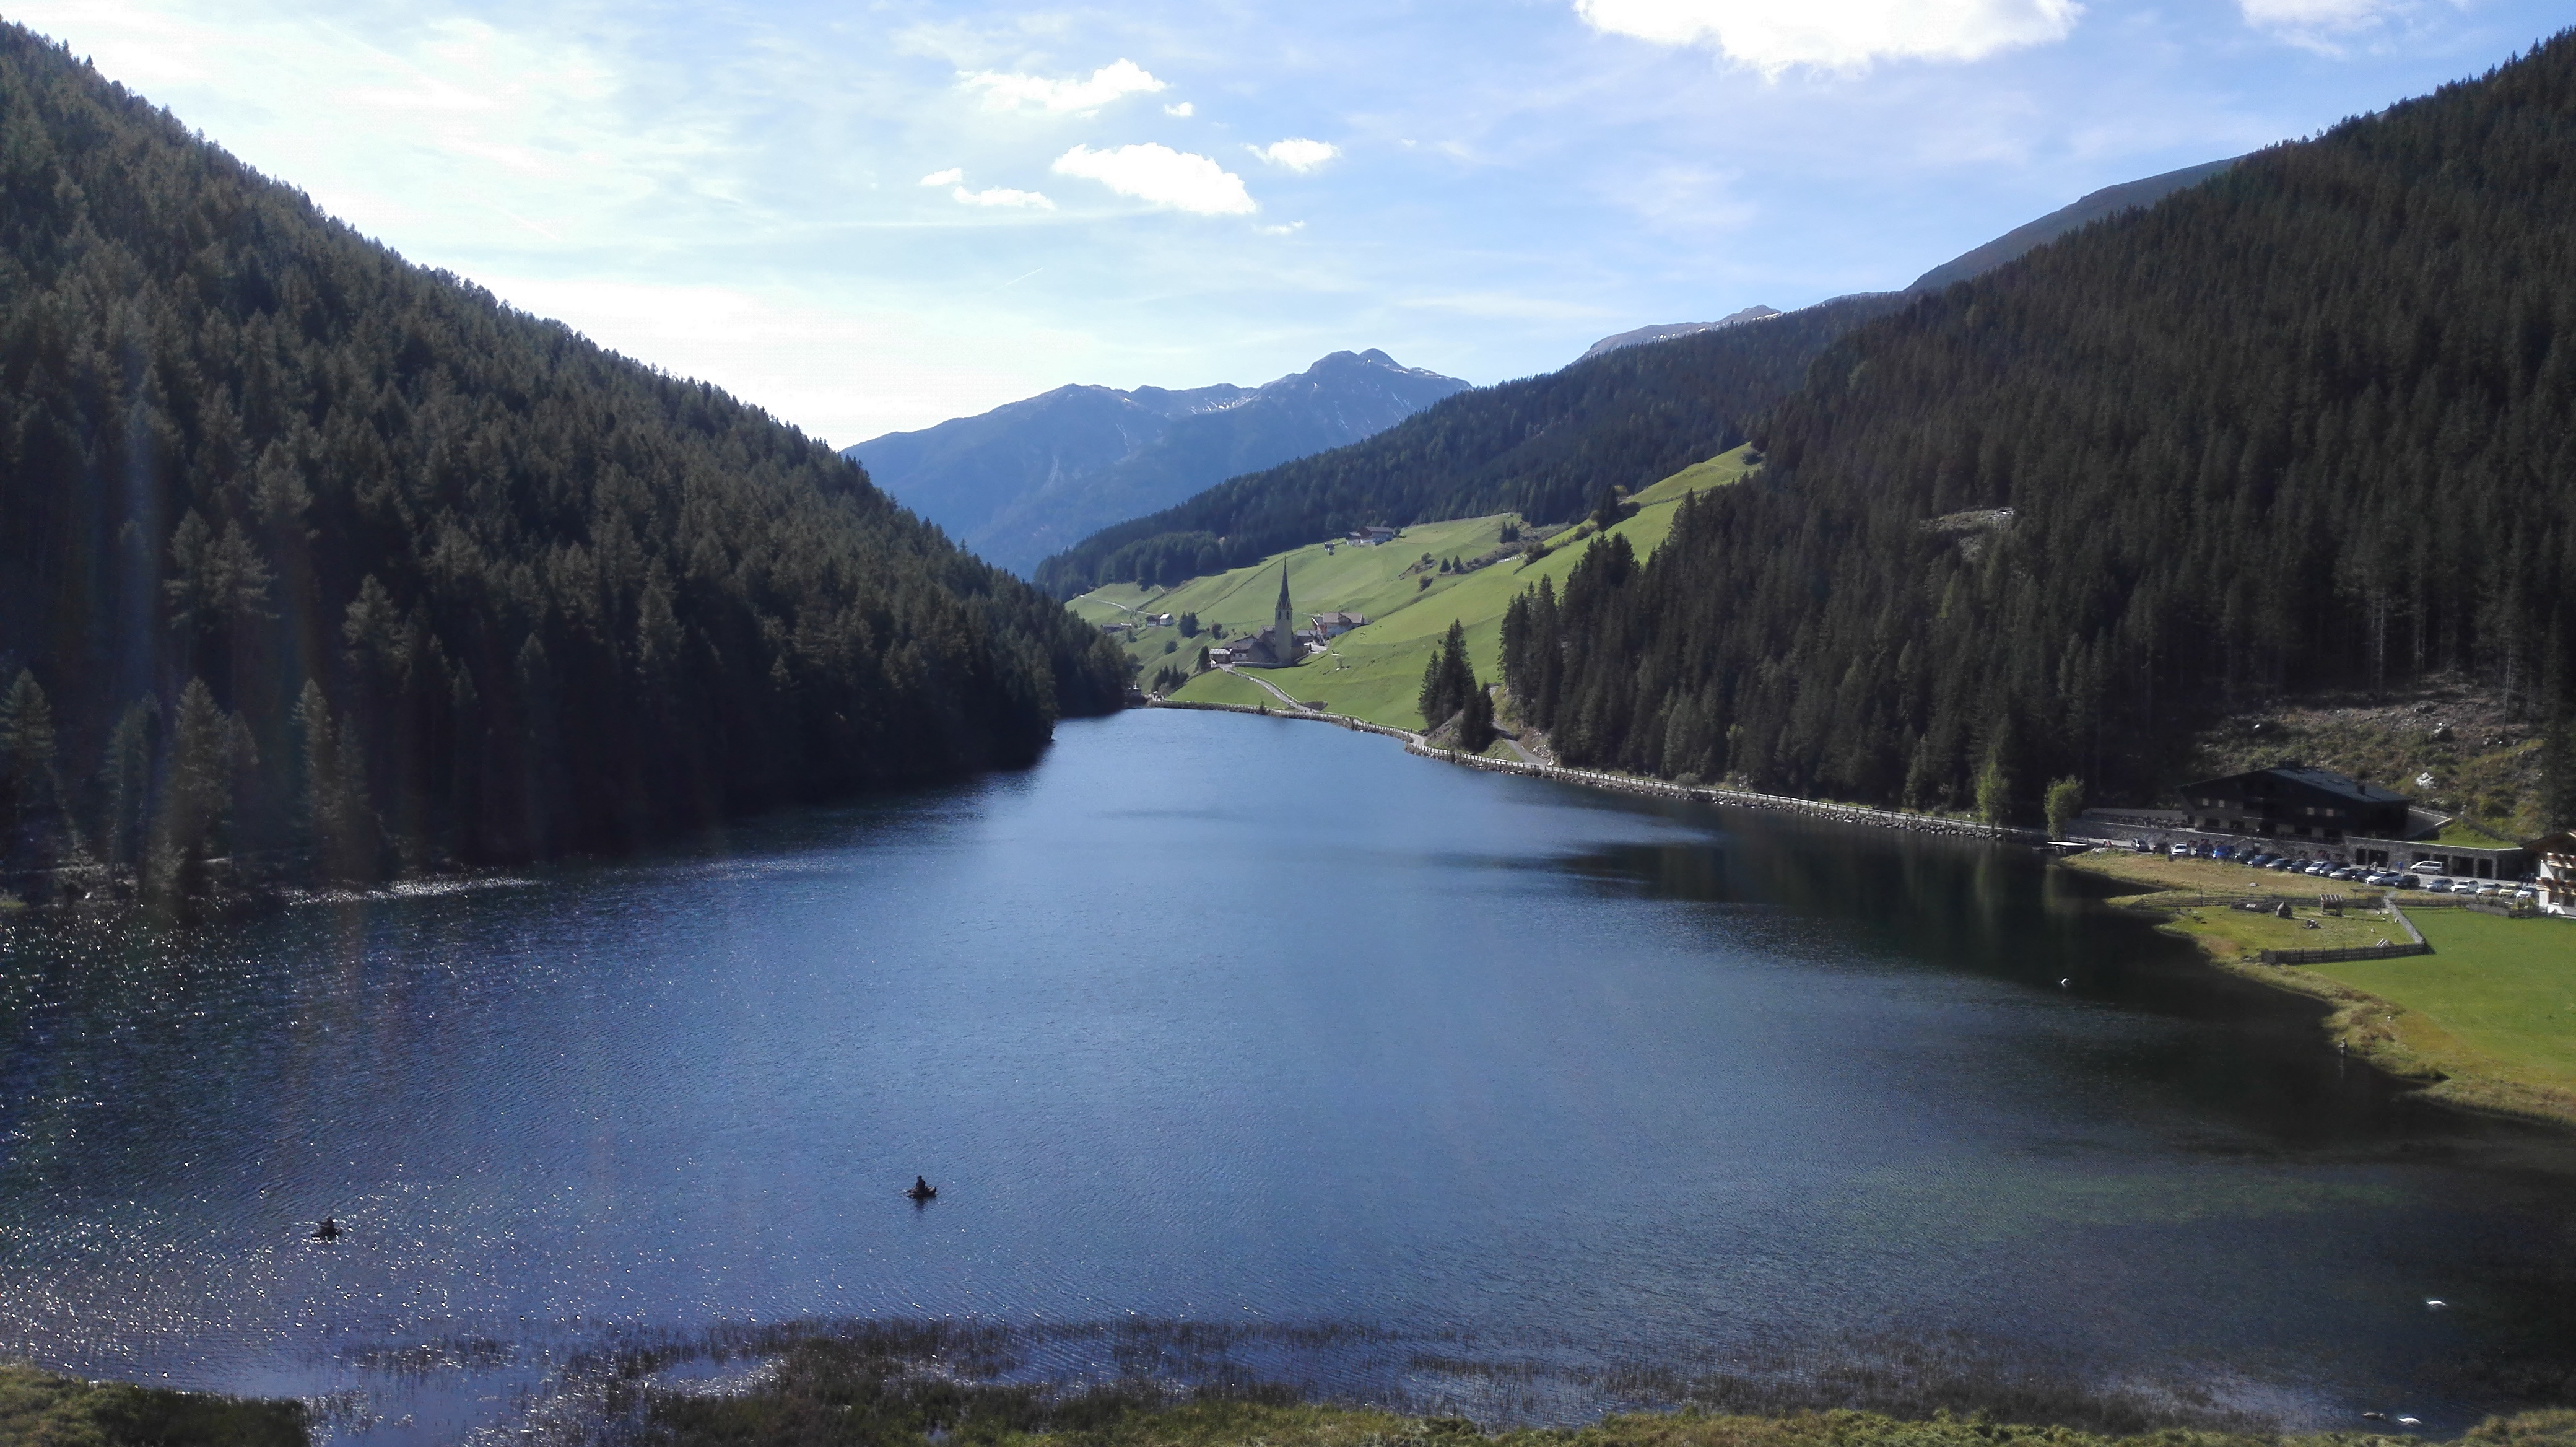
\includegraphics[scale=0.045]{img/Durnholz.jpg}%
 		\caption{Lake Durnholz where the run takes place.}\label{fig:durnholz}%
 	\end{center}%
\end{figure}
\begin{figure}[ht]%
 	\begin{center}%
 		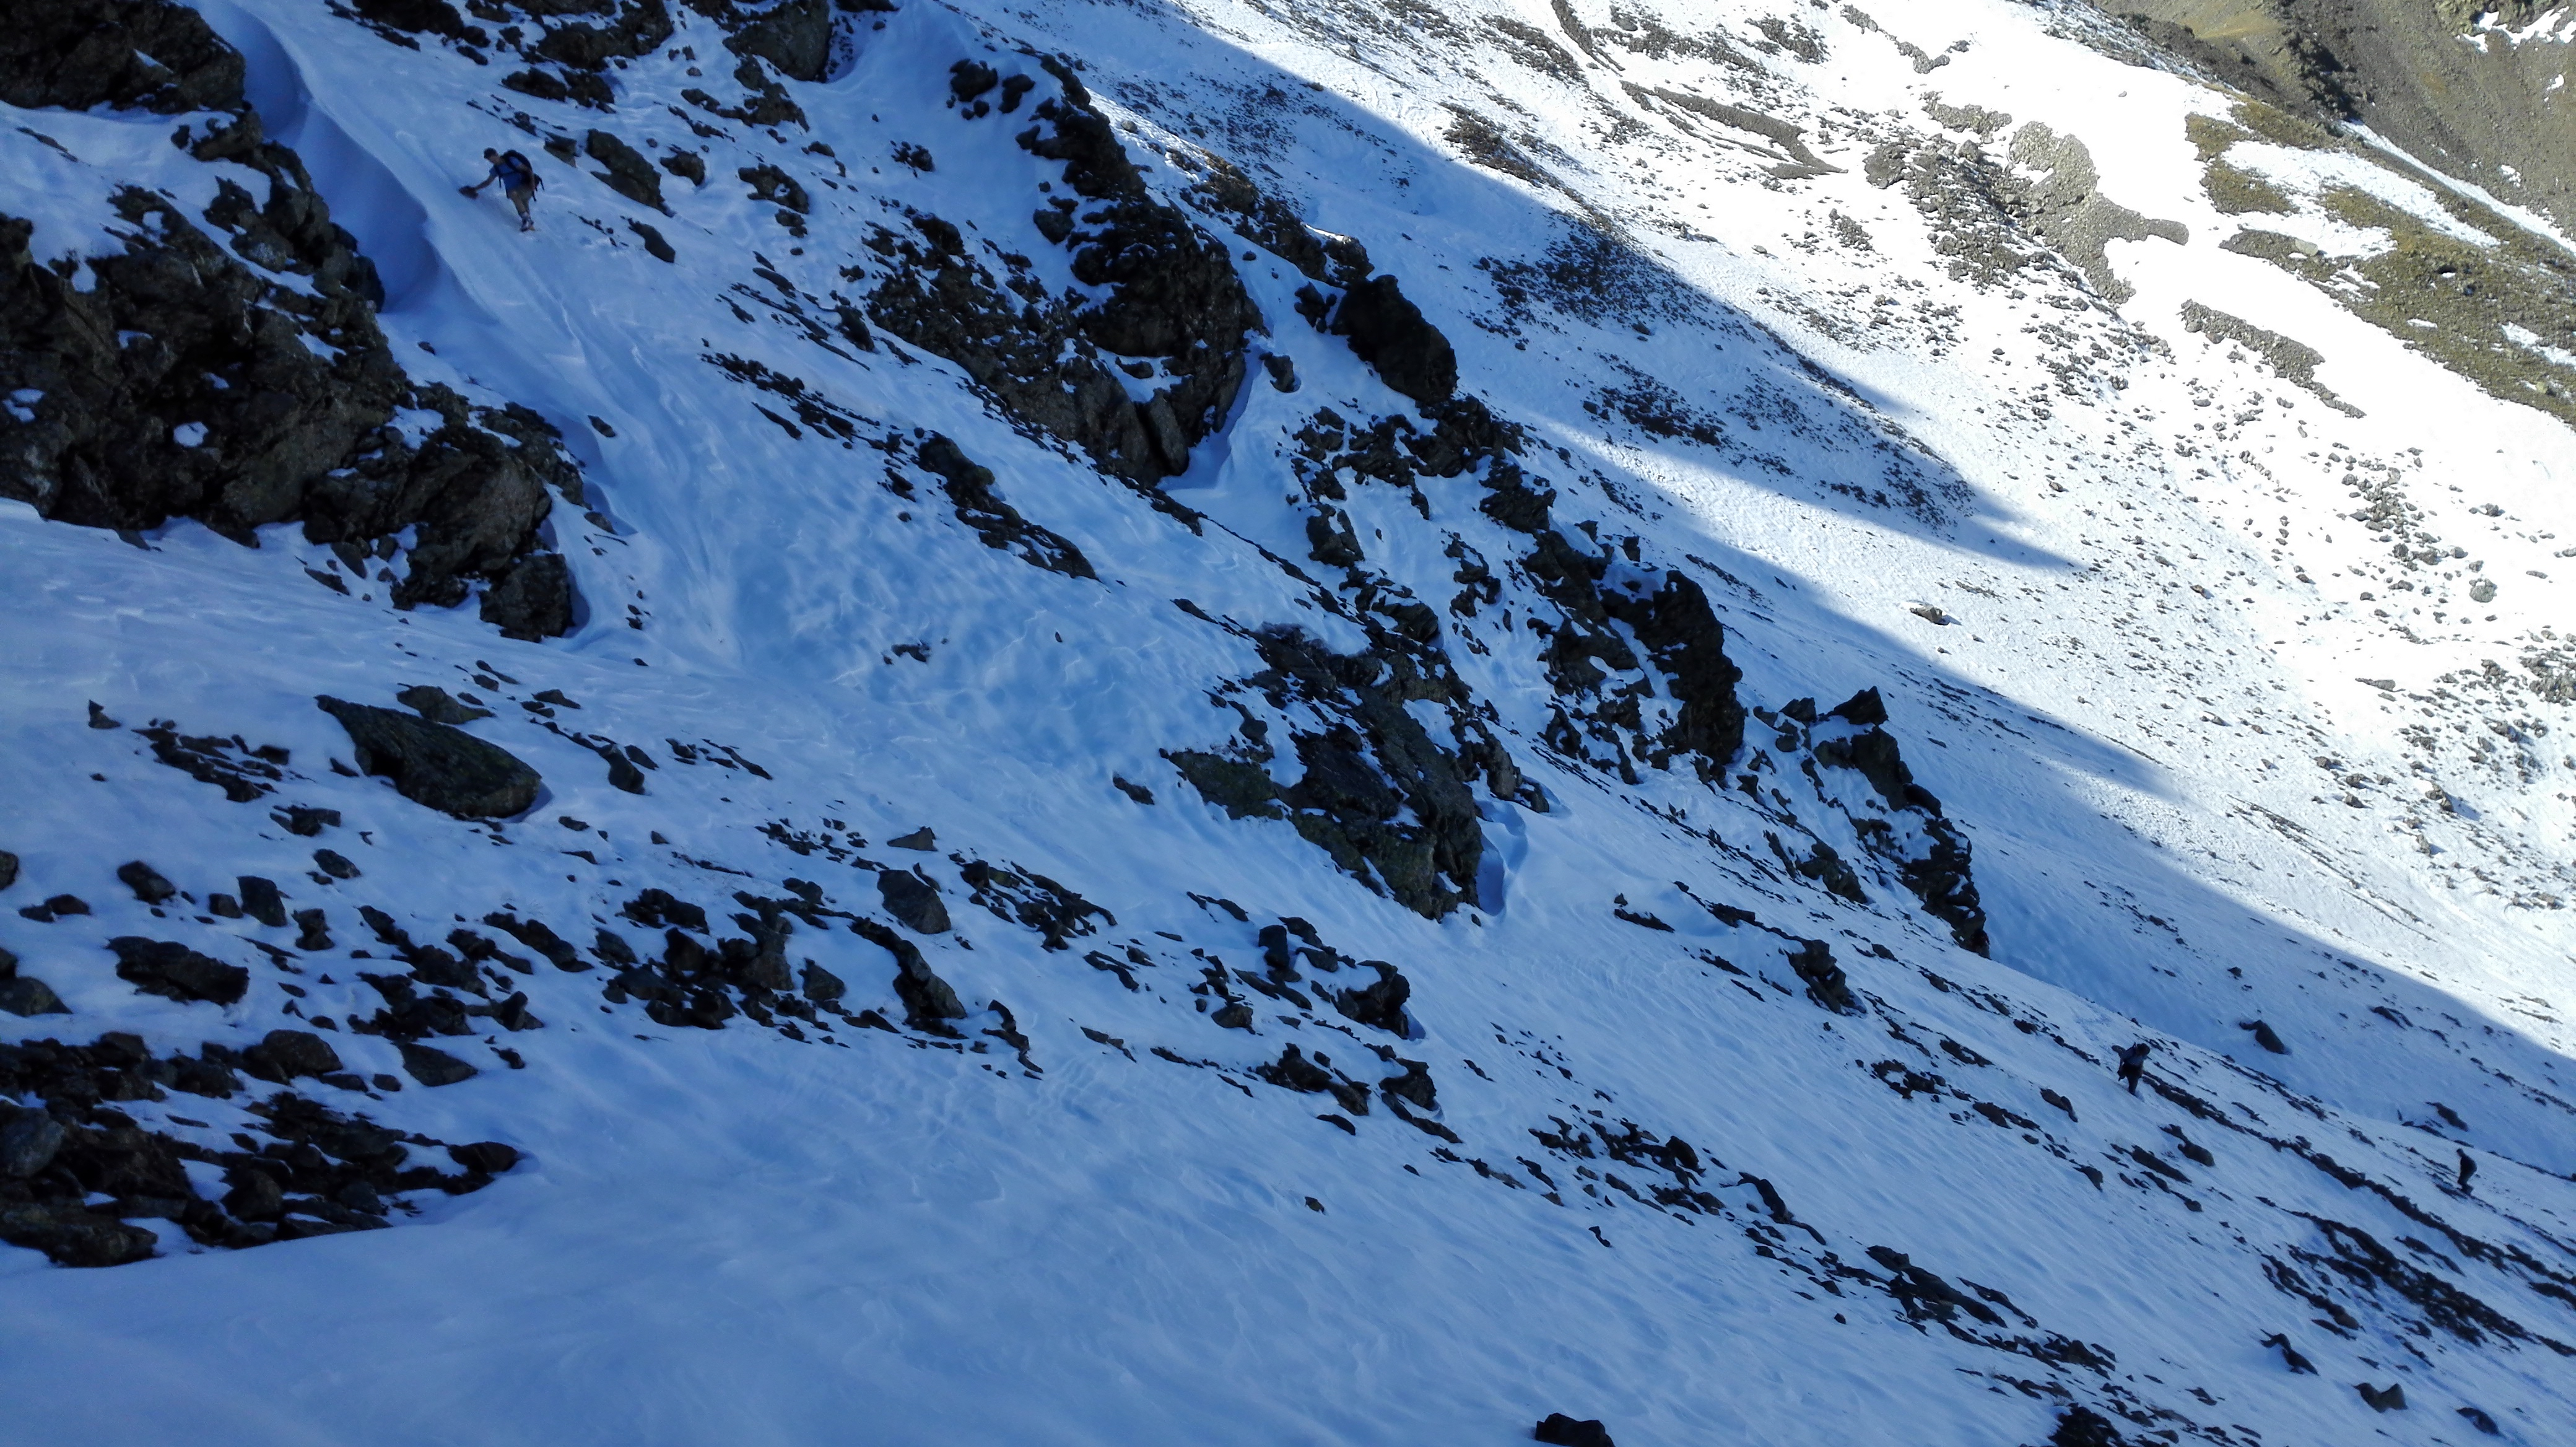
\includegraphics[scale=0.045]{img/Snow.jpg}%
 		\caption{It can get quite snowy during hikes.}\label{fig:Snow}%
 	\end{center}%
\end{figure}
